% Efficiency Scaling Figure for PAC Learning Bounds
\begin{figure}[htbp]
\centering
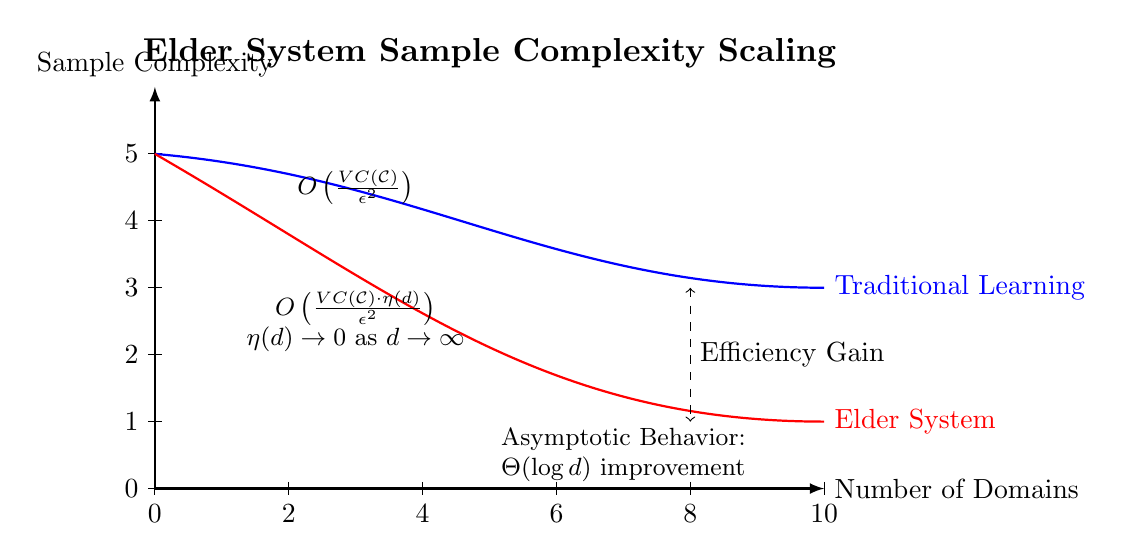
\begin{tikzpicture}[scale=0.85]
    % Define styles
    \tikzset{
        axis/.style={thick, ->, >=latex},
        traditional/.style={thick, blue},
        elder/.style={thick, red},
        annotation/.style={font=\small}
    }
    
    % Draw axes
    \draw[axis] (0,0) -- (10,0) node[right] {Number of Domains};
    \draw[axis] (0,0) -- (0,6) node[above] {Sample Complexity};
    
    % Draw tick marks on x-axis
    \foreach \x in {0,2,4,6,8,10} {
        \draw (\x,0.1) -- (\x,-0.1) node[below] {$\x$};
    }
    
    % Draw tick marks on y-axis
    \foreach \y in {0,1,2,3,4,5} {
        \draw (0.1,\y) -- (-0.1,\y) node[left] {$\y$};
    }
    
    % Draw traditional learning curve
    \draw[traditional] (0,5) to[out=-5, in=180] (10,3) 
        node[right] {Traditional Learning};
    
    % Draw Elder system learning curve
    \draw[elder] (0,5) to[out=-30, in=180] (10,1) 
        node[right] {Elder System};
    
    % Add annotations
    \node[annotation, align=center] at (3,4.5) {$O\left(\frac{VC(\mathcal{C})}{\epsilon^2}\right)$};
    \node[annotation, align=center] at (3,2.5) {$O\left(\frac{VC(\mathcal{C}) \cdot \eta(d)}{\epsilon^2}\right)$\\$\eta(d) \to 0$ as $d \to \infty$};
    
    % Add efficiency gain illustration
    \draw[<->, dashed] (8,3) -- (8,1) node[midway, right] {Efficiency Gain};
    
    % Add asymptotic behavior
    \node[annotation, align=left] at (7,0.5) {Asymptotic Behavior:\\$\Theta(\log d)$ improvement};
    
    % Add title
    \node[align=center, font=\bfseries, scale=1.2] at (5,6.5) {Elder System Sample Complexity Scaling};
\end{tikzpicture}
\caption{Efficiency scaling of the Elder system compared to traditional learning approaches. As the number of domains increases, the Elder system achieves significantly better sample complexity due to its knowledge transfer, hierarchical structure, and universal principle extraction capabilities. The efficiency factor $\eta(d)$ decreases as the number of domains increases, leading to a logarithmic improvement $\Theta(\log d)$ in the asymptotic limit. This represents a fundamental advantage of the Elder architecture for multi-domain learning problems.}
\label{fig:efficiency_scaling}
\end{figure}